\subsection{Expresión general de un filtro digital}
    En muchas aplicaciones del procesado de señales es necesario diseñar dispositivos o algoritmos que realicen operaciones sobre las señales y que los englobaremos bajo la denominación genérica de sistemas.

    Un sistema opera sobre una señal de entrada o excitación según una regla preestablecida, para generar otra señal llamada salida o respuesta del sistema a la  excitación propuesta y que puede simbolizarse

    \begin{equation}
      y[n] = T(x[n])
    \end{equation}

    donde $T$ simboliza la transformación, operador o procesado realizado por el sistema sobre la señal $x$ para producir la señal $y$ (ver Fig. \ref{fig:esquemaFiltro}). Una de las motivaciones más fuertes para el desarrollo de herramientas generales para el análisis y diseño de sistemas es que proviniendo a menudo de aplicaciones muy diferentes tienen descripciones matemáticas similares.

    \begin{figure}
      \centering
      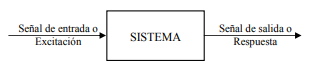
\includegraphics[width=0.4\textwidth]{../images/esquemaFiltro.png}
      \caption{Esquema del sistema, señal de entrada y respuesta o salida del sistema}
      \label{fig:esquemaFiltro}
    \end{figure}

    Existen varias maneras de representar un sistema, ya que muchos sistemas reales están construidos como interconexiones de varios subsistemas, tal como se grafica en la Fig. \ref{fig:interconexionSistema}.

    \begin{figure}
      \centering
      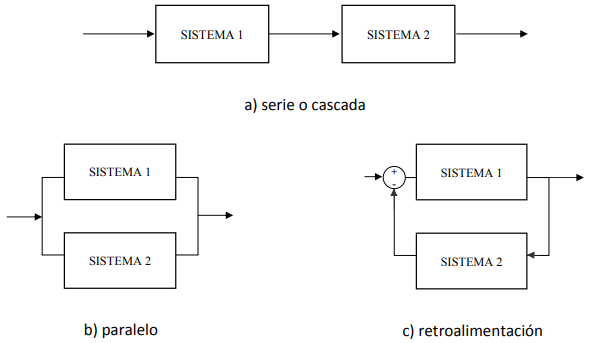
\includegraphics[width=0.5\textwidth]{../images/interconexionSistema.png}
      \caption{Interconexión de sistemas}
      \label{fig:interconexionSistema}
    \end{figure}

    Existen dos métodos básicos para el análisis del comportamiento o respuesta de un sistema lineal a una determinada entrada. Un primer camino se basa en obtener la solución de la ecuación entrada‐salida del sistema que en general tiene la forma de las ecuaciones en diferencias lineales a coeficientes constantes $a_{m}$, $b_k$

    \begin{equation}
      \sum_{m=0}^{N_a - 1}{a_m y[n-m]} = \sum_{k=0}^{N_b - 1}{b_k x[n-k]}
      \label{eq:defFiltro}
    \end{equation}

    siendo $N_a$ y $N_b$ los órdenes máximos de las diferencias en la ecuación correspondiente a la entrada y a la saldia del sistema.

    El segundo método para el análisis del comportamiento del sistema reside en la aplicación del principio de superposición y consiste en descomponer la señal de entrada en una suma pesada de señales elementales las cuales se escogen de manera que sea conocida la respuesta del sistema a las mismas. Siguiendo esta línea, una señal a tiempo discreto puede visualizarse como una secuencia pesada de impulsos unitarios

    \begin{equation}
      x[n] = \sum_{k=-\infty}^{\infty}{x[k] \cdot \delta [n - k] }
    \end{equation}

    Aplicando la propiedad de superposición de los SLIT (Sistemas Lineales e Invariantes en el Tiempo) (Oppenheim y Willsky, 1983), se puede determinar la salida del sistema ante una cierta entrada de la siguiente manera

    \begin{equation}
      y[n] = \sum_{k=-\infty}^{\infty}{x[k] \cdot h[n-k]}
    \end{equation}

    siendo $h[n]$ la respuesta o salida del sistema ante una entrada equivalente a un impulso unitario $\delta [n]$ denominada /respuesta al impulso del sistema/. El segundo miembro de la expresión representa el producto de convolución de la señal de entrada $x[n]$ y la respuesta al impulso del sistema $h[n]$; esto es

    \begin{equation}
      y[n] = x[n] * h[n] = h[n] * x[n]
    \end{equation}

    Tanto en el caso continuo como en el caso discreto, la respuesta al impulso del sistema LTI presenta las siguientes propiedades

    \begin{itemize}
      \item Sin memoria: $h[n]=0$ para $n \neq 0$.
      \item Causal: $h[n]=0$ para $n<0$.
      \item Invertible: dado $h[n]\: \exists \:h'[n]\::\:h[n]*h'[n]=\delta[n]$.
      \item Estable: $\sum_{k=-\infty}^{\infty}{|h[n]|<\infty}$
    \end{itemize}

    Existen otras formas de representar un filtro, todas estas equivalentes a la respuesta al impulso unitario de sistema SLIT, sin embargo muchas veces conviene más una u otra representación. En el caso aplicar la transformada Z, a la \ref{eq:defFiltro} se obtiene la función de transferencia del sistema (Oppenheim y Willsky, 1983; Proakis y Manolakis; 1996; Oppenheim y Schafer, 1999)

    \begin{equation}
      H(z) = \frac{\sum_{k=0}^{N_b-1}{b_k z^{-k}}}{\sum_{m=0}^{N_a-1}{a_m z^{-m}}}
      \label{eq:6}
    \end{equation}

    donde $z=A\exp(j\Omega)$ es la variable compleja en forma polar. Particularmente si el modulo $A=1$, la expresión de la Ec. \ref{eq:6} se reduce a la respuesta en recuencia del sistema a través de la transformada de Fourier a tiempo discreto (Oppenheim y Willsky, 1983; Proakis y Manolakis; 1996; Oppenheim y Schafer, 1999):

    \begin{equation}
      y[n] = \sum_{k=0}^{N_b-1}{b_k x[n-k]} - \sum_{m=1}^{N_a-1}{a_m y[n-m]}
    \end{equation}

    donde los coeficientes $a_m$ y $b_k$ son los coeficientes que definen el filtro, por lo tanto el diseño consiste en calcularlos. Como regla general se suele dejar el término $a_0=1$.

%%% Local Variables:
%%% mode: latex
%%% TeX-master: "../main"
%%% End:
